%\listfiles
\documentclass[tg]{mdtuffs}
% um tipo específico de monografia pode ser informado como parâmetro opcional:
%\documentclass[tese]{mdtuffs}
% a opção `openright' pode ser usada para forçar inícios de capítulos
% em páginas ímpares
% \documentclass[openright]{mdtuffs}
% para gerar uma versão frente-e-verso, use a opção 'twoside':
% \documentclass[twoside]{mdtuffs}
%\usepackage{hyperref}	
%\usepackage{breakurl}
\usepackage[T1]{fontenc}        % pacote para conj. de caracteres correto
\usepackage{fix-cm} %para funcionar corretamente o tamanho das fontes da capa
\usepackage{times, color,xcolor}       % pacote para usar fonte Adobe Times e cores
\usepackage[utf8]{inputenc}   % pacote para acentuação
\usepackage{graphicx}  % pacote para importar figuras
%\usepackage[brazil]{babel}   
\usepackage{enumerate}
\usepackage{amsmath,latexsym,amssymb} %Pacotes matemáticos
\usepackage[%hidelinks%, 
            bookmarksopen=true,linktoc=none,colorlinks=true,
            linkcolor=black,citecolor=black,filecolor=magenta,urlcolor=blue,
            pdftitle={Título da Dissertação ou Trabalho ....},
            pdfauthor={Nome Autor Sobrenome},
            pdfsubject={Projeto/Trabalho de Conclusão de Curso},
            pdfkeywords={Monografia, Modelo, LaTeX}
            ]{hyperref} %hidelinks disponível no pacote hyperref a partir da versão 2011-02-05  6.82a
%Nesse caso, hidelinks retira os retângulos em volta dos links das referências

%Definição de minha autoria pra funcionar as XML
%\def\lnl#1#2{{\scriptsize\bfseries #1}\hspace{#2em}}

%---------------------------------------------------
% Definições dos XML
%---------------------------------------------------
\usepackage{verbatim}
\usepackage{listings}
%\usepackage[usenames,dvipsnames]{color}
	%\def\mlnl#1#2{{\scriptsize\bfseries #1}\hspace{#2em}}

%---------------------------------------------------
% Definições dos Algoritmos
%---------------------------------------------------
	\usepackage[portuguese,ruled,linesnumbered]{algorithm2e}
	\usepackage{etoolbox}
	\makeatletter
	\patchcmd{\@algocf@start}{%
		\begin{lrbox}{\algocf@algobox}%
	}{%
	  \rule{0.\textwidth}{\z@}%
	  \begin{lrbox}{\algocf@algobox}%
	  \begin{minipage}{1.\textwidth}%
	}{}{}
	\patchcmd{\@algocf@finish}{%
	  \end{lrbox}%
	}{%
	  \end{minipage}%
	  \end{lrbox}%
	}{}{}
	\makeatother

	\SetAlFnt{\tt}
	
	\SetKwFunction{FRecurs}{FnRecursive}%
%-------------------------------------------------

     
\sloppy
%%Margens conforme MDT 1ª edição, arrumar diretamente no mdtuffs.cls para funcionar a opção twoside *PENDENTE*
\usepackage[inner=30mm,outer=20mm,top=30mm,bottom=20mm]{geometry} 

%==============================================================================
% Se o pacote hyperref foi carregado a linha abaixo corrige um bug na hora
% de montar o sumário da lista de figuras e tabelas
% Se o pacote não foi carregado, comentar a linha %
%==============================================================================

%%=============================================================================
%% Trampa para corrigir o bug do hyperref que redefine o caption das figuras e das
%% tabelas, n�o colocando o nome ``Figura'' antes do n�mero do mesmo na lista
%%=============================================================================

\makeatletter

\long\def\@caption#1[#2]#3{%
  \expandafter\ifx\csname if@capstart\expandafter\endcsname
                  \csname iftrue\endcsname
    \global\let\@currentHref\hc@currentHref
  \else
    \hyper@makecurrent{\@captype}%
  \fi
  \@ifundefined{NR@gettitle}{%
    \def\@currentlabelname{#2}%
  }{%
    \NR@gettitle{#2}%
  }%
  \par\addcontentsline{\csname ext@#1\endcsname}{#1}{%
    \protect\numberline{\csname fnum@#1\endcsname ~-- }{\ignorespaces #2}%
  }%
  \begingroup
    \@parboxrestore
    \if@minipage
      \@setminipage
    \fi
    \normalsize
    \expandafter\ifx\csname if@capstart\expandafter\endcsname
                    \csname iftrue\endcsname
      \global\@capstartfalse
      \@makecaption{\csname fnum@#1\endcsname}{\ignorespaces#3}%
    \else
      \@makecaption{\csname fnum@#1\endcsname}{%
        \ignorespaces
        \ifHy@nesting
          \expandafter\hyper@@anchor\expandafter{\@currentHref}{#3}%
        \else
          \Hy@raisedlink{%
            \expandafter\hyper@@anchor\expandafter{%
              \@currentHref
            }{\relax}%
          }%
          #3%
        \fi
      }%
    \fi
    \par
  \endgroup
}

\makeatother

%==============================================================================
% Identificação do trabalho
%==============================================================================
\title{Título}

\author{Sobrenome}{Nome}
%Descomentar se for uma "autora"
%\autoratrue

\course{Curso de Ciência da Computação}
\altcourse{Curso de Ciência da Computação}

%não usado por enquanto
\institute{Ciência da Computação}
\degree{Bacharel em Ciência da Computação}

% Número do TG (verificar na secretaria do curso)
% Para mestrado deixar sem opção dentro do {}
\trabalhoNumero{}

%Orientador
\advisor[Prof.]{Dr.}{Sobrenome}{Nome}
%Se for uma ``orientadora'' descomentar a linha baixo
%\orientadoratrue

%Co orientador, comentar se não existir
%\coadvisor[Prof.]{Drª.}{Pereira}{Maria Regina}
%\coorientadoratrue %Se for uma ``Co-Orientadora''

%Avaliadores (Banca)
\committee[Dr.]{Sobrenome}{Nome}{UFFS}
\committee[Me.]{Sobrenome}{Nome}{UFFS}

% a data deve ser a da defesa; se nao especificada, são gerados
% mes e ano correntes
\date{1}{Janeiro}{2014}

%Palavras chave
%\keyword{Dissertação} 
%\keyword{Modelo}
%\keyword{LaTeX}

%%=============================================================================
%% Início do documento
%%=============================================================================
\begin{document}

%%=============================================================================
%% Capa e folha de rosto
%%=============================================================================
\maketitle

%%=============================================================================
%% Catalogação e Folha de aprovação
%%=============================================================================
%Somente obrigatório para dissertação, para TG, remover as linhas	77	%
%Como a CIP vai ser impressa atrás da página de rosto, as margens inner e outer	
%devem ser invertidas.
%\newgeometry{inner=20mm,outer=30mm,top=30mm,bottom=20mm}	
%\makeCIP{email@email.com} %email do autor		
%\restoregeometry

%Se for usar a catalogação gerada pelo gerador do site da biblioteca comentar as linhas
%acima e utilizar o comando abaixo
%\includeCIP{CIP.pdf}

%folha de aprovação
\makeapprove

%%=============================================================================
%% Dedicatória (opcional)
%%=============================================================================
%\clearpage
%\begin{flushright}
%\mbox{}\vfill
%{\sffamily\itshape Texto da dedicatória ......}
%\end{flushright}

%%=============================================================================
%% Agradecimentos (opcional)
%%=============================================================================
%\chapter*{Agradecimentos}
%Agradecimentos


%%=============================================================================
%% Epígrafe (opcional)
%%=============================================================================
%\clearpage
%\begin{flushright}
%\mbox{}\vfill
%{\sffamily\itshape
%``Frase da epígrafe'' \\ }
%--- \textsc{Autor da frase}
%\end{flushright}


%%=============================================================================
%% Resumo
%%=============================================================================
\begin{abstract}
Resumo...
\end{abstract}

%%=============================================================================
%% Abstract
%%=============================================================================
% resumo na outra língua
% como parametros devem ser passados o titulo, o nome do curso,
% as palavras-chave na outra língua, separadas por vírgulas, o mês em inglês
%o a sigla do dia em inglês: st, nd, th ...
\begin{englishabstract}
{Title}
{Bachelor of Computer Science}
{Keywords1. Keyword2}
{March}
{st}
Abstract... 

\end{englishabstract}

%% Lista de Ilustrações (opc)
%% Lista de Símbolos (opc)
%% Lista de Anexos e Apêndices (opc)

%%=============================================================================
%% Lista de figuras (comentar se não houver)
%%=============================================================================
\listoffigures

%%=============================================================================
%% Lista de tabelas (comentar se não houver)
%%=============================================================================
\listoftables

%%=============================================================================
%% Lista de Apêndices (comentar se não houver)
%%=============================================================================
%\listofappendix

%%=============================================================================
%% Lista de Anexos (comentar se não houver)
%%=============================================================================
%\listofannex

%%=============================================================================
%% Lista de abreviaturas e siglas
%%=============================================================================
 %o parametro deve ser a abreviatura mais longa
%\begin{listofabbrv}{UbiComp}
%   \item [BNF] \textit{Backus-Naur Form}
 %  \item [UbiComp] Computação Ubíqua
%\end{listofabbrv}


%%=============================================================================
%% Lista de simbolos (opcional)
%%=============================================================================
%Simbolos devem aparecer conforme a ordem em que aparecem no texto
% o parametro deve ser o símbolo mais longo
%\begin{listofsymbols}{teste}
 % \item [$\varnothing$] vazio
 % \item [$\Gamma$]  Gama
 % \item [$\forall$] Para todo
%\end{listofsymbols}

%%=============================================================================
%% Sumário
%%=============================================================================
\tableofcontents


%%=============================================================================
%% Início da monografia
%%=============================================================================
\setlength{\baselineskip}{1.5\baselineskip}

%Adiciona cada capitulo
\chapter{Introdução}

Texto da introdução.
\chapter{Referencial Teórico}
Neste capítulo serão apresentados os principais conceitos e as relações que definem a problemá́tica.
\section{Arquitetura de software}
%AS - O que é
O conceito de Arquitetura de Software surgiu em resposta ao aumento da complexidade dos sistemas de software existentes, este vem sendo agregado por de segmentos como: redes, servidores, bancos de dados, interfaces de usuário, dependências de requisitos, atributos de qualidade de software, atributos de segurança, redundância, replicação e escalabilidade \cite{hanschke2015integrating}.

\cite{bass2007software} apresenta a arquitetura de software como sendo um resultado de um conjunto de decisões de negócio aliadas à decisões técnicas, sendo que este resultado é diretamente influenciado pelo ambiente em que a arquitetura está sendo projetada para ser executada. O autor também afirma que a arquitetura é diretamente influenciada pelos \textit{stakeholders} (proprietário, cliente, desenvolvedor, gestor de projeto, tomadores de decisão do produto entre outros) envolvidos no projeto e interessados na construção do mesmo, diferentes \textit{stakeholders} podem exigir determinados requisitos como: baixo custo de desenvolvimento, grande variedade de funcionalidades, fácil customização, otimização para determinados hardwares. É compreensível que um sistema com o mínimo de requisitos de qualidade (performance, disponibilidade, compatibilidade, uso de recursos e usabilidade para o usuário) deva atender a todos os requisitos de qualidade impostos inclusive pelos \textit{stakeholders} mas, esta será uma árdua tarefa à ser balanceada pelo arquiteto de software no momento do design.

\cite{babar2014making} define a arquitetura de software como:
\begin{itemize}
\item Um conjunto de elementos arquiteturais (ex: informações, processamentos, conexões entre requisitos, modelagens de dados e processos).
\item A forma como estes elementos agem como princípios para guiar  o relacionamento entre elementos e suas propriedades.
\item A análise racional para a escolha de elementos e sua interação com todo o conjunto do sistema.
\end{itemize}  

%AS - Por que é importante?%
A antecipação da arquitetura de software de sistemas pode trazer uma série de vantagens \cite{babar2013agile}, sistemas complexos tipicamente possuem arquiteturas complexas e quando estas forem compostas por partes originadas de sistemas de terceiros podem gerar a necessidade de ajustes e adequações. 

As tendências recentes na descrição da arquitetura de software como um conjunto de decisões de design com diagnóstico das próprias decisões tem destacado a importância da análise racional na realização e descrição das decisões de design tomadas. \cite{babar2009software}

Segundo \cite{hanschke2015integrating}, é importante considerar a realização da documentação do projeto compreendendo os elementos no design de soluções de software efetivas. Este processo compõe definir arquitetura em diversas perspectivas e níveis de abstração, ponderando sobre todas as várias propriedades da arquitetura, assegurando que esta seja concebível com um conjunto de implementações que irão atender os requisitos do sistema, evoluindo e integrando arquiteturas complexas. A realização da arquitetura de software no processo e ciclo de vida de desenvolvimento de software é considerada a etapa mais desafiadora à ser definida pois é considerada como uma solução traduzida em sistema que deve ser projetada antecipadamente da fase de projeto. 

Considerando a arquitetura de software no contexto do ambiente corporativo, existem três razões fundamentais onde pode ser observada a sua importância \cite{bass2007software}:

\begin{enumerate}
    \item \textit{Comunicação entre os stakeholders.} A arquitetura de software representa uma abstração de um sistema que pode ser utilizada por todos os stakeholders como base para a compreensão mútua, negociação, consenso e comunicação. 
    \item \textit{Decisões antecipadas de design.} A arquitetura de software é capaz de apresentar decisões de requisitos de maneira antecipada e estas ações diminuem o peso sobre o desenvolvimento de maneira à antecipar a resolução de impedimentos que podem surgir através de uma análise detalhada do requisito.
    \item \textit{Abstração transferível do sistema.} Os conhecimentos em torno da arquitetura de um sistema e a sua propriedade intelectual costumam ser mantidos sob a guarda de poucos ou até um único envolvido no projeto. A documentação de arquitetura bem estruturada permite a transferência deste conhecimento para outros \textit{stakeholders} além da replicação e transferência para outros projetos.
    
\end{enumerate}
%AS -  dependência em relação aos requisitos 

\cite{babar2013agile} Para compreender e validar um conjunto de requisitos pode ser necessário o uso da modelagem com a compreensão de uma série de soluções de arquitetura sendo que muitas delas podem ser inviáveis devido à determinadas restrições de requisitos. 

\cite{hanschke2015integrating} afirmaram que uma série de esforços já foram realizados aprimorando processos para suportar o design da arquitetura de sistemas complexas, modelagem, refinação e conexão arquitetural de elementos em design detalhado das implementações.  Em relação ao processo, é necessário identificar e capturar os requisitos funcionais e não funcionais do projeto e então realizar a tentativa de definir uma arquitetura que cumpra estes requisitos.

A composição do escopo de recursos e custo de um sistema ao projetar uma arquitetura baseada em um sistema existente pode facilitar em grande parte o processo devido à existencia dos componentes chave que já podem ser facilmente antecipados e compreendidos \cite{babar2013agile}.

Também é compreensível que requisitos possam ser alternados por outros à partir do momento em que seja identificado a impossibilidade de realização do mesmo  \cite{babar2013agile}.  

\cite{hanschke2015integrating} ressalta que na prática e em ambientes reais as soluções arquiteturais são acompanhadas de diversas restrições, existem importantes pontos que devem ser observados como: quais requisitos podem ser atendidos e como eles devem ser atendidos, principalmente tratando-se de requisitos não funcionais.

Um fator crítico na antecipação da arquitetura é o potencial de excesso de planejamento da arquitetura e consequente excesso de investimento em um requisito que pode nunca ser utilizado esta situação pode ser comparada à situações onde existe um baixo investimento em infra-estrutura onde o sistema poderá falhar na execução do serviço corretamente durante a sua execução \cite{grundy2012guest}. 

%AS - impacto da arquitetura nas decisões sobre a fase de desenvolvimento, 

\cite{beck2001manifesto} também revela que um erro crítico é a impossibilidade de adaptar-se ao grande número de mudanças ou re-priorização de requisitos que podem vir à ocorrer com o aumento da experiência dos usuários após a utilização do sistema. A antecipação de design de arquitetura implica na manutenção de alguns requisito gerais, funcionais e não funcionais, para que permaneçam consistentes ao longo de todo o ciclo de vida do projeto para que o relacionamento entre requisitos e arquitetura deve torne-se uma única evolução. 


\subsection{Orientação à objetos}

Na concepção da orientação à objetos, Alan Kay imaginou objetos como recursões do conceito de um computador, sendo cada um desdes objetos responsável pela correta realização de pequenas tarefas próprias sendo este sistema passível de uma melhor compreensão após ser observado em maior escala, funcionando em conjunto com diversos outros objetos integralmente \cite{reenskaug2009dci}. O autor afirma que a Orientação à Objetos é altamente distribuída, sendo de fato um paradigma complexo de delinear em situações em que ocorrem concorrência e paralelismo.

O paradigma da orientação a objetos é um conceito que pode ser aplicado independente da linguagem de programação utilizada. O desenvolvimento de softwares utilizando a orientação à baseado em objetos é fundamentalmente\cite{rumbaugh1991object} Dentro deste paradigma são apresentados alguns conceitos que compõem a própria orientação à objetos:

\begin{enumerate}
% \item \textit{Comunicação entre os stakeholders.}
\item \textit{Abstração:} É a visão geral de determinados componentes de um sistema com o objetivo de interligá-los à outros componentes, omitindo detalhes específicos, concentrando-se apenas em seu comportamento e interação no sistema como um todo. Segundo \cite{rumbaugh1991object} a abstraçào consiste na percepção dos aspectos fundamentais de uma entidade ou seja, antes de analisar sua implementação, concentrar-se no que o objeto faz e o que é. Através da abstração é possivel obter a liberdade de tomar decisões evitando influenciar em detalhes específicos do objeto antes de sua implementação.

\end{enumerate}

\subsection{Conceitos }

%TO-DO complementar

\subsection{Modelo-visão-controlador}

%TO-DO

\section{Arquitetura de software com métodos ágeis}

% surgimento

Com o decorrer do tempo a comunidade de desenvolvimento de software iniciou uma reação buscando suprir a necessidade de respostas mais rápidas aos stakeholders, sendo mais ativo no desenvolvimento de funcionalidades das quais o usuário realmente percebe propostas de valor e após o surgimento dos métodos ágeis os arquitetos de software questionaram-se sobre o como estes métodos se encaixariam nas práticas de arquitetura de software. \cite{babar2013agile} ressalta que a inflexibilidade dos métodos normais tem um propósito. Obter um planejamento antecipado permite uma ótima predição do projeto desde que os requisitos não mudem com frequência, além de facilitar a coordenação de um grande número de times de desenvolvimento.

% distancia arquitetura e ágil

Segundo \cite{abrahamsson2010agility} o distanciamento entre os métodos ágeis e a arquitetura de software refere-se ao grande tempo desprendido na antecipação de problemas relacionados à arquitetura, enquanto os métodos ágeis procuram ser adaptativos, tomando decisões conforme a percepção de mudança de requisitos. 

Na literatura, vários estudos apontam problemas relacionados a evolução do projeto de software e dificuldades com a arquitetura. \cite{waterman2015much} aponta que negligências de atividades de arquitetura podem acontecer dependendo dos valores buscados na entrega e que podem ser diretamente influenciados pelo tempo e orçamento do projeto. \cite{martini2015investigating} e \cite{bellomo2013study} afirmam que as limitações de tempo e orçamento podem resultar na tomada de decisões rápidas visando a entrega de funcionalidades, o que afeta diretamente o tempo dedicado ao planejamento e desenvolvimento de uma arquitetura adequada.

Um arquiteto de software que projeta uma arquitetura de sistema com datas reais de entrega e prazos apertados irá tomar um determinado conjunto de decisões porém, o mesmo arquiteto ao projetar um sistema similar onde as datas de entrega e prazos podem ser facilmente atendidas, certamente tomará decisões diferentes. Da mesma maneira criar um design de arquitetura com os mesmos requisitos de hardware, recursos e interfaces atuais não tem o mesmo impacto que desenvolver uma arquitetura para um sistema que será entregue e executada daqui a 5 anos \cite{bass2007software}.

Dentro da própria comunidade de pessoas envolvidas em processos de desenvolvimento e design de softwares existem lados rigorosamente definidos  uma incompatibilidade entre a agilidade e arquitetura. Neste contexto é necessário refletir sobre as seguintes perguntas: Quanto de arquitetura eu devo desenvolver versus quanto eu devo flexibilizar durante o projeto? Como e quando eu devo refatorar projetos? Quanto de arquitetura eu devo formalizar em documentos? Devo revisar minha arquitetura? Se sim, quando?
\cite{babar2013agile}

\section{Os métodos ágeis e a arquitetura de software}

%  Valores e princípios dos métodos ágeis versus Métodos ágeis Scrum e XP  versus Arquitetura de software

% enfatizar arquitetura não é valor percebido pelo cliente

\section{Documentação de arquitetura nos métodos ágeis}

\section{Práticas que permitem melhorar a arquitetura nos métodos ágeis}

\section{Refatoração de arquitetura}

Tratando-se de sistemas de software, a expansão do mesmo com novas funcionalidades e mudanças sem o devido acompanhamento conduzirá o surgimento de uma arquitetura com falhas que podem ser difíceis de eliminar. 

\cite{babar2013agile} definem que a refatoração é um método de melhorar a estrutura interna do sistema sem alterar o comportamento externo, introduzindo a refatoração sistemática e os padrões de refatoração é possível ajudar engenheiros de software a prover soluções lidando com necessidades decorrentes da refatoração além de auxiliar evitando a erosão sistema.
Nenhuma aplicação deveria ser construída de única vez,  deveria entretanto ser pensada e desenvolvida em pequenas partes onde a cada iteração um requisito ou pequena parte é definido arquiteturalmente e em seguida implementado.

Devido à falta de ferramentas que suportem diretamente a refatoração de arquitetura, é possível utilizar ferramentas existentes que auxiliem ao menos em parte do processo de refatoração como por exemplo, na identificação de problemas de arquitetura na fase de análise ou mediante análise de código já implementado.

Segundo \cite{babar2013agile} arquitetos de software podem reconhecer a necessidade de melhorias de arquitetura quando o código apresentar as seguintes características: 
    \begin{itemize}
        \item Código duplicado
        \item Métodos com muitas de linhas.
        \item Uso de switchs em excesso.
    \end{itemize}

Além das características detalhadas de código que caracterízam as chamadas \textit{architecture smells} (termo utilizado para a presença de "cheiros ruins" na arquitetura, onde há a necessidade de aplicar refatorações para resolver possíveis problemas) ainda existem outros artefatos que podem ser identificados na arquitetura em si que podem caracterizar a necessidade de refatoração.

\begin{description}

\item[Artefatos duplicados:] Há uma dificuldade em definir quanta replicação é aceitável ou benéfica, e que tipo de repetições de código são consideradas problemas de arquitetura. Não há uma resposta concreta para isso, depende do contexto onde o principio DRY \textit{(Don't Repeat Yourself)} deve ou não ser aplicado.

\item[Papeis indefinidos:] O nomes dos componentes devem explicar as responsabilidades para que os envolvidos no projeto entendam facilmente. As responsabilidades devem ser designados para componentes individuais e não sobre múltiplos componentes. Da mesma maneira um componente deve ter apenas uma responsabilidade e deve faze-la bem.

\item[Arquitetura muito complexa:] Complexidades acidentais levam abstrações desnecessárias. Essas abstrações levam a softwares inexpressivos, Como componentes supérfluos ou dependências. Arquitetura deve ser simplista da melhor maneira possível.

\item[Tudo centralizado:] É necessário evitar ao máximo dentro do sistema, arquiteturas \textit{hub} devem ser evitadas pois podem acabar sintetizando tudo em um único ponto de falha.

\item[Utilizar soluções caseiras ao invés de melhores práticas:] É necessário evitar reinventar a roda. A probabilidade de métodos já conhecidos e testados serem melhores que novas práticas é alta.

\item[Arquiteturas muito genéricas:] Sistemas genéricos podem vir a ser complexos se exigirem muitas configurações por serem muito e o excesso de abstração pode aumentar a manutenção.

\item[Estruturas com comportamentos assimétricos:]
A simetria é o indicador de uma boa qualidade de arquitetura, existem dois tipos de simetria: simetria de comportamento e estrutural. Assimetria de comportamento lida com as funcionalidades no início de sua atividade, e assegura que todas as ações iniciem e terminem de uma maneira adequada. A assimetria estrutural garante que todas as questões sejam resolvidas utilizando soluções padronizadas.

\item[Ciclo de dependência:]
Caso haja componentes que dependam uns dos outros, existe a possibilidade de haver impactos na testabilidade e modificabilidade do sistema.

\item[Violações de design:]
As violações de design, como evitar utilizar os padrões corretos do projeto e utilização de padrões diferentes para atender as soluções dos problemas podem diminuir a expressividade do sistema.

\item[Particionamento inadequado de funcionalidades:]
O particionamento inadequado pode causar complexidade adicional não desejada na arquitetura.

\item[Dependências desnecessárias:]
Para reduzir a complexidade número de dependências deve ser minimizado. Dependências que são pouco utilizadas ou pareçam desnecessários devem ser removidas.

\item[Dependências implícitas:]
Quando as implementação do sistema contendo dependências que não são viáveis no modelo arquitetural, estas devem ser removidas pois podem causar obrigações desnecessárias. Implementações com mudanças podem causar erros caso o engenheiro de software não esteja atento a essas dependências implícitas. Um exemplo frequente de dependências implícitas é o uso frequente de variáveis globais. Também conhecidas como padrão sigleton.

\end{description}

A refatoração de um componente não crítico de arquitetura não deve ser aplicado imediatamente após a data de release. Porém, se uma refatoração em especifico não é aplicada em uma iteração por algum motivo, está se torna um débito de design e precisa ser resolvida na próxima iteração, já artefatos de arquitetura que não foram verificados na sprint atual devem ser mantido no backlog para serem analisado em seguida.

\subsection{Principais obstáculos na refatoração de arquitetura}
\begin{description}
\item[Organização e gestão:] 
Os stakeholders do projeto consideram as novas funcionalidades como sendo as mais importantes.
A premissa de que “a arquitetura de software deve ser feita corretamente no primeiro momento para que não haja problemas futuramente” ignora o fato de que existem constantes mudanças na arquitetura inclusive no momento da criação de novas funcionalidades.
Primeiramente, os engenheiros de software não conhecem todos os requerimentos (pelo menos não com todos os detalhes). 
Além disso o design de todo o processo não funciona. O que torna crescimento passo à passo do sistema como a melhor alternativa porém, o crescimento passo à passo requer uma constante avaliação de qualidade de todos os artefatos de design que também precisam de refatoração de arquitetura. Um problema comum é que a refatoração de arquitetura apenas pode provar seu valor após a conclusão do projeto podendo assim não haver nenhum retorno do investimento à curto prazo porem, é comprovado que a negligência de padrões de qualidade é muito mais custosa do que a inserção de verificações de qualidade periódicas. De acordo com a lei de Conway, a organização dita a arquitetura portanto, uma má organização leva à uma má arquitetura.

\item[Processo de desenvolvimento:]
O processo de refatoração precisa ser explicitamente integrado no processo de desenvolvimento geral. Do contrário, o gerenciamento do projeto não planejará recursos suficientes para os objetivos da refatoração,
os \textit{stakeholders} e testadores devem estar cientes da refatoração para que as mudanças possam ser validadas.

\item[Tecnologia e ferramentas:]
Devido à falta de ferramentas que suportem diretamente a engenharia de refatoração de arquitetura, o processo de ver feito manualmente mediante análise da estrutura atual e avaliação da reimplementação conforme a mudança do requisito de qualidade em questão.

\item[Aplicabilidade:]
Se a erosão de design da arquitetura de software do projeto desenvolvido for grande ao ponto de que a refatoração resolverá apenas os sintomas e não as causas, e reengenharia ou até a reconstrução do projeto pode ser mais adequada e eficiente.
\end{description}


% - (o que é, quais as dificuldades e obstáculos, )

\subsection{Refatoração versus reengenharia de arquitetura}

\section{Trabalhos relacionados}

\subsection{Artigo relacionado 1}

\subsection{Artigo relacionado 2}
\chapter{Metodologia}

A pesquisa consiste em propor um processo que auxilie na refatoração de arquitetura em projetos de software que utilizam métodos ágeis.

O plano de pesquisa a ser utilizado seguirá orientações de \cite{dias2010developing} através uma abordagem baseada em evidências, esta inclui as seguintes atividades principais:
\begin{enumerate}[(a)]

\item Identificar estudos preliminares: condução de revisão sistemática da literatura com a finalidade de identificar estudos relacionados a refatoração de arquitetura nos métodos ágeis, que tratem de métodos ou práticas utilizados e problemas vivenciados.

\item Proposta da abordagem: proposta de uma abordagem para auxiliar na atividade de refatoração de arquiteturas nos métodos ágeis: definição de atividades a serem desenvolvidas, processo a ser seguido e recomendações de forma de adequação aos princípios ágeis. A proposta será construída baseada nas evidências. 
% to-do obetidas na etapa A (revisão da literatura)

\item Validação da proposta com especialista: Considerando que a proposta apresenta tanto contribuições práticas quanto teórica, a validação da proposta será realizada com especialista da academia e profissionais da indústria. Como representantes da academia serão entrevistados 2 pesquisadores da área de Engenharia de Software e como representantes da indústria serão entrevistados 2 consultores sobre métodos ágeis. Para realização da validação será utilizada a técnica de grupos focados. O planejamento das reuniões, a condução das reuniões e forma de análise dos dados, seguirão as recomendações de \cite{ribeiro2003gruposfocados}.

\item Validação da proposta através da aplicação em uma situação real: realização de uma pesquisação numa empresa que apresenta o contexto de pesquisa estudado. Para realização da pesquisa-ação serão seguidas as recomendações de \cite{dos2008colaboraccao}. As métricas utilizadas para a validação durante o processo de pesquisa-ação serão levantadas com base no acompanhamento de \textit{sprints} realizadas pelo desenvolvimento da empresa.

% , sendo considerados para este levantamento os seguintes relatórios:
    
%   \begin{itemize}
%         \item Diagrama acumulativo de fluxo de tarefas.
%         \item Gráfico de controle para medição de estabilidade de métricas.
%         \item Gráfico de velocidade para histórias implementadas.
%         \item Gráfico burndown para apresentação de alterações de escopo não planejado.
%     \end{itemize}  
    
\end{enumerate}

As validações à serem aplicadas utilizam métricas que já são monitoradas atualmente no ambiente de desenvolvimento da empresa em questão onde a pesquisa-ação será realizada, desta maneira será possível avaliar com maior embasamento o impacto que a aplicação da melhoria proposta tratá ao ambiente de desenvolvimento e consequentemente às métricas de acompanhamento. A figura \ref{fig:estrategia_pesquisa} apresenta a metodologia de pesquisa proposta, que inclui as seguintes atividades principais:
\begin{figure}[ht]
\centering
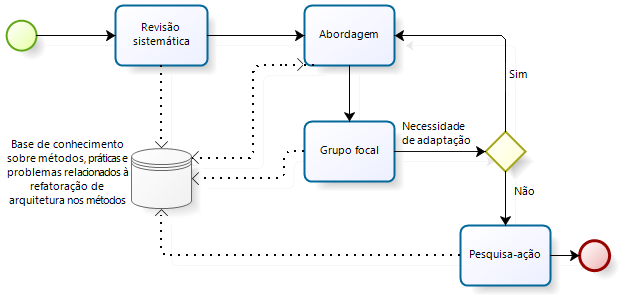
\includegraphics[scale=0.90]{figuras/estrategia_pesquisa}
\caption{ Estratégia de pesquisa}
% \resizebox{!}{0.3cm}{}
\label{fig:estrategia_pesquisa}
\end{figure}


\chapter{Trabalhos Relacionados}

~\cite{hofmeister2007general}.

5 métodos de arquitetura de software industriais

1 - Attribute-Driven Design
ADD utiliza da decomposição da regra de negócio (processo) de modulos do sistema para criação do design da arquitetura. Requisitos como atributos de qualidade e requisitos funcionais do módulo já devem estar definidos.
Etapas:
a) definição de diretrizes arquiteturais, momento onde é definido o que é ou não importante nos requisitos minimos do modulo
b) definição de um padrão que atenda as diretrizes
c) instancie modulos e aloque funcionalidades de casos de uso, criando views
d) defina interface e modulos filhos, revisando todo o design para ter certeza que nada foi esquecido

2 - Siemens 4 views
(continuar...)




\cite{pressman2009engenharia}


\cite{babar2013agile}

PAG. 21 - Muitas pessoas envolvidas na área tem lados rigorosamente definidos, defendendo uma incompatibilidade entre a agilidade e arquitetura. 


PAG 29 - Com o surgimento do agir engenheiros se preocuparam em com os métodos ágeis se encaixavam em outros métodos e práticas de engenharia.


O agil é uma resposta do mundo para necessidade de projetos que sejam mais responsivos aos interessados no projeto, mais rapidez no desenvolvimento de funcionalidades ao qual usuários se interessam.


Grande pergunta é: quanto de arquitetura eu devo desenvolver versus quanto eu devo flexibilizar durante o projeto? Como e quando eu devo relatora? Quanto de arquitetura eu devo formalizarem documentos? Deve revisar minha Arquitetura? Se sim, quando?


A flexibilidade dos métodos normais não era pra nada. Ter um bom plano antecipado facilita a predição (desde que os requisitos no mudem muito) E facilita a gestão de grandes times.


Os métodos ágeis por outro lado, rejeitam o planejamento preferem trabalho em 
equipe, comunicação frente-a-frente, Flexibilidade adaptação..


Na opinião do doutor, projetos de sucesso requerem uma mistura das duas estratégias.



PAG 44 - Tal sugere que uma refatoração sistemática pode ajudar a prevenir erosões arquiteturais através da avaliação do designer do software existente antes de chamar novos artefatos no sistema atual.


















pag. 88 - cap. 3 - Refactoring Software Architectures (TODO O CAPÕTULO 3)


PG 63 - Na engenharia de software, mudanças são regras e não exceções.

PG64 - a refatoração é um método de melhorar a estrutura sem alterar o comportamento externo[1]. Introduzindo a refatoração sistemática e os padrões de refatoração é possível ajudar engenheiros de software a prover soluções lidando com necessidades decorrentes da refatoração. E também é possível auxiliar evitando a erosao sistema


PG65 - nenhuma aplicação deve ser construída de única vez mas deve ser pensado em pequenas partes onde a cada iteração um requisito ou pequena parte é definido arquiteturalaumente


PG66 - Como engenheiros podem reconhecer que eles precisa melhorar a estrutura de uma implementação?

A existência de:

- código duplicado,
- métodos dúzias de linhas,
- usos de switchs frequentemente


PG68 - 
Artefatos duplicados - Há uma dificuldade em definir quanta replicação é aceitável ou benéfica, e que tipo de repetições de código são consideradas problemas de arquitetura. Não há uma resposta concreta para isso, depende do contexto onde o principio DRY deve ou não ser aplicado.

Papeis indefinidos - Os números componentes devem explicar as responsabilidades para que os envolvidos no projeto entendam facilmente. As responsabilidades devem ser designados para componentes individuais E não sobre múltiplos componentes. Do contrário esses componentes sofreram. Da mesma maneira um componente deve ter apenas uma responsabilidade e deve fazer bem.


Arquitetura muito complexa - complexidades acidentais levam abstrações desnecessárias. Essas abstrações levam a softwares inexpressivos, Como componentes supérfluos ou não coisas. Arquitetura deve ser simplista da melhor maneira possível.

Tudo centralizado: É necessário evitar· dentro do sistema, arquiteturas hub ou spoke devem ser evitados pois sintetizando tudo em um único ponto de falha.

Utilizar soluções caseiras ao invés de melhores práticas
: É necessário evitar reinventar a roda. A probabilidade E métodos já conhecidos e testados serem melhores que novas práticas é alta.

Arquiteturas muito genéricas: sistema sistema podem vir a ser complexo se exigindo muitas configurações por serem muito genéricos E o excesso de abstração pode aumentar a manutenção.


Estruturas com comportamentos assimétricos:

A simetria é o indicador de uma boa qualidade de arquitetura, existem dois tipos de simetria: simetria de comportamento estrutural. Assimetria de comportamento lidar com as funcionalidades no início de sua atividade, E assegura que todas as ações iniciem e terminem de uma maneira adequada. 


Ciclo de dependência:
Caso haja componentes que dependam uns dos outros, existe a possibilidade de haver impactos na testabilidade que modificabilidade do sistema.

Violações de design:
As violações de design, Como evitar utilizar os padrões corretos do projeto O Utilização de padrões diferentes para atender as soluções dos problemas podem diminuir a expressividade do sistema.

Particionamento inadequado de funcionalidades:
Podem causar complexidade acidental

Dependências desnecessárias:
Para reduzir a complexidade número de dependências deve ser minimizado. Dependências que são pouco utilizadas ou pareçam desnecessários devem ser removidas.

Dependências implícitas:
Quando as implementação do sistema contendo dependências que não são viáveis no modelo arquitetural, estas devem ser removidas pois podem causar obrigações desnecessárias. Implementações com mudanças podem causar erros caso o engenheiro de software não esteja atento a essas dependências implícitas. Um exemplo frequente de dependencias implícitas é o  uso frequente de variáveis globais. Também conhecidas como padrão sigleton.

PG 73- 

1. avaliação de arquitetura:
Identifique os problemas de design, Ou Seja, a habilidade da arquitetura de alcançar os termos de qualidade buscados

2. priorização:
Prioriza As questões determinando a prioridade dos componentes afetados.

3. Seleção:
Para cada problema na lista(iniciando com maior prioridade) Como usar as seguintes atividades:
	3.1 Padrão de refatoração adequado. Neste contexto, apropriado significa que o padrão escolhido resolveu problema interna e externamente
	3.2 Se existe mais de um padrão, escolha O que mais se adapta ao design E que melhor trarão impacto positivo na qualidade.
	3.3 cara esse padrão não exista volto para o design da arquitetura convencional.

4. verificação da qualidade: 
	Para cada aplicação de refatoração verifique Como o sistema foi afetado.
	4.1 abordagem formal: prova com métodos formais que a estruturação não alterou comportamento anterior. Abordagens formais são úteis em sistemas de tempo real.
	4.2 avaliação da arquitetura: façam uma avaliação geral
	

Devido à falta de ferramentas que suportem diretamente a refatoração de arquitetura, ao menos é possível utilizar ferramentas existentes que  auxiliem em parte do processo de refatoração, por que auxiliem Na identificação de problemas de arquitetura na fase de análise.

A retratação de um componente não crítico de arquitetura não deve ser aplicado imediatamente após a data de release. Porém, Se uma refatoração em especifico não é aplicada em uma iteração por algum motivo, está se torna um débito de design e precisa ser resolvida na próxima iteração. No set de scrum, programas de arquitetura que não são verificados na sprint atual Deve ser mantido no backlog.


PG75 - 	Exemplos de padrões de refatoração de arquitetura

Quebrar ciclos de dependencia - 
É possível utilizar técnicas como injeção de dependência ou tentar inverter uma ou mais dependências buscando resolver os ciclos.

Divisão em subsistemas - 

O nível de acoplamento e coesão pode ser utilizado como indicador para dividir ou combinar sub-sistemas.

pg78 - OBSTACULOS NA REFATORAÇÃO DE ARQUITETURA

- Organização e gestao 
Os stakeholders do projeto consideram as novas funcionalidades como sendo as mais importantes.
A premissa de que “a arquitetura de software deve ser feita corretamente no primeiro momento para que não haja problemas futuramente” ignora o fato de que existem constantes mudanças na arquitetura inclusive no momento da criação de novas funcionalidades.
Primeiramente, os engenheiros de software não conhecem todos os requerimentos (pelo menos não com todos os detalhes). 
Além disso o design te todo o processo não funciona. O que torna crescimento passo à passo do sistema como a única alternativa.
Porém o crescimento passo à passo requer uma constante avaliação de qualidade de todos os artefatos de design que também precisam de refatoração de arquitetura.

Um problema comum é que a refatoração de arquitetura apenas pode provar seu valor após a conclusão do projeto. Podendo não haver nenhum retorno do investimento, porem é comprovado que a negligencia de padrões de qualidade é muito mais custosa do que a inserção de verificações de qualidade periódicas.

De acordo com a lei de Conway, a organização dita a arquitetura portanto, má organização leva à uma má arquitetura.


- Processo de desenvolvimento
O processo de relatora
cão precisa ser explicitamente integrado no processo de desenvolvimento geral. Do contrário, o gerenciamento do projeto não planejará recursos suficientes para os objetivos da refatoração.
os stakeholder e testadores devem estar cientes da refatoração para que as mudanças possam ser validadas.

- Tecnologia e ferramentas
Devido à falta de ferramentas que suportem diretamente a engenharia de refatoração de arquitetura, o processo de ver feito manualmente.

- Aplicabilidade
Se a erosão de design for grande ao ponto de que a refatoração resolverá apenas os sintomas e não as causas, e reengenharia ou até a reconstrução pode ser mais adequada e eficiente.



 

pat. 107 - referÍncias do cap. 3 























PAG 161 - A refatoração de arquitetura é uma etapa interativa para implementação da variabilidade (habilidade do software de ser adaptado)

PAG 169 - Uma técnica é usada no memomento apropriado, e não é mais utilizada quando não for mais útil.

Refatoração continua foca na resolução do problema, sendo que as atividades de análise devem preceder as atividades de recuperação, Em casa ideal, a refatoração executado continuamente, Pois é mais fácil fazer pequenas mudanças Durante o processo de desenvolvimento do que fazer uma grande mudança em determinado ponto. Porém, grandes refatorações nem sempre podem ser evitados, [52,58,43]









\cite{hofmeister2007general}



\setlength{\baselineskip}{\baselineskip}

%%=============================================================================
%% Referências
%%=============================================================================
%\bibliographystyle{abbrv}
%\bibliography{referencias/referencias}
\bibliographystyle{abnt}
\bibliography{referencias/referencias}



%IMPORTANTE: Se precisar usar alguma seção ou subseção dentro dos apêndices ou
%anexos, utilizar o comando \tocless para não adicionar no Sumário
%Exemplos: 
% \tocless\section{Histórico}
%%=============================================================================
%% Apêndices
%%=============================================================================
%\appendix
%\include{capitulos/apendicea}
%\include{capitulos/apendiceb}

%%=============================================================================
%% Anexos
%%=============================================================================
%\annex
%\include{capitulos/anexoa}

\end{document}
